%****************************************************************************%
%* DIET User's Manual JXTA chapter file                                     *%
%*                                                                          *%
%*  Author(s):                                                              *%
%*    - Sylvain DAHAN (dahan@lifc.univ-fcomte.fr)                           *%
%*                                                                          *%
%*  This file is part of DIET 2.1.                                          *%
%*                                                                          *%
%*  Copyright (C) 2000-2003 ENS Lyon, LIFC, INSA and INRIA,                 *%
%*                          all rights reserved.                            *%
%*                                                                          *%
%*  Since DIET is open source, free software, you are free to use, modify,  *%
%*  and distribute the DIET source code and object code produced from the   *%
%*  source, as long as you include this copyright statement along with      *%
%*  code built using DIET.                                                  *%
%*                                                                          *%
%*  Redistribution and use in source and binary forms, with or without      *%
%*  modification, are permitted provided that the following conditions      *%
%*  are met.                                                                *%
%*                                                                          *%
%*  Redistributions of source code must retain the copyright notice below   *%
%*  this list of conditions and the following disclaimer. Redistributions   *%
%*  in binary form must reproduce the copyright notice below, this list     *%
%*  of conditions and the following disclaimer in the documentation         *%
%*  and/or other materials provided with the distribution. Neither the      *%
%*  name of ENS Lyon nor the names of its contributors (LIFC, INSA Lyon,    *%
%*  INRIA) may be used to endorse or promote products derived from this     *%
%*  software without specific prior written permission.                     *%
%*                                                                          *%
%*  THIS SOFTWARE IS PROVIDED BY THE COPYRIGHT HOLDERS AND CONTRIBUTORS     *%
%*  "AS IS" AND ANY EXPRESS OR IMPLIED WARRANTIES, INCLUDING, BUT NOT       *%
%*  LIMITED TO, THE IMPLIED WARRANTIES OF MERCHANTABILITY AND FITNESS       *%
%*  FOR A PARTICULAR PURPOSE ARE DISCLAIMED. IN NO EVENT SHALL THE          *%
%*  REGENTS OR CONTRIBUTORS BE LIABLE FOR ANY DIRECT, INDIRECT,             *%
%*  INCIDENTAL, SPECIAL, EXEMPLARY, OR CONSEQUENTIAL DAMAGES (INCLUDING,    *%
%*  BUT NOT LIMITED TO, PROCUREMENT OF SUBSTITUTE GOODS OR SERVICES ;       *%
%*  LOSS OF USE, DATA, OR PROFITS ; OR BUSINESS INTERRUPTION) HOWEVER       *%
%*  CAUSED AND ON ANY THEORY OF LIABILITY, WHETHER IN CONTRACT, STRICT      *%
%*  LIABILITY, OR TORT (INCLUDING NEGLIGENCE OR OTHERWISE) ARISING IN ANY   *%
%*  WAY OUT OF THE USE OF THIS SOFTWARE, EVEN IF ADVISED OF THE             *%
%*  POSSIBILITY OF SUCH DAMAGE.                                             *%
%*                                                                          *%
%****************************************************************************%

\chapter{Multi-MA extension}
\label{ch:multiMAextension}

The hierarchical organization of DIET is efficient when the set of resources is
shared by few individuals. However, the aim of grid computing is to share
resources between several individuals. In that case, the DIET hierarchy become
inefficient. The Multi-MA extension has been implemented to resolve this
issue. This chapter explains the different scalability issues of grid computing
and how to use the multi-MA extension to deal with them.

\section{Function of the Multi-MA extension}

The use of a monolithic architecture become more and more difficult when the
number of users and the number of resources grow simultaneously. When a user
try to resolve a problem, without the multi-MA extension, DIET looks for the
better SeD that can resolve it. This search involves the fact that each SeD has
to be queried to run a performance prediction as described in
section~\ref{sec:solvepb}.

The need to query every SeD that can resolve a problem is a serious
scalability issue. To avoid it, the multi-MA extension proposes to interconnect
several MA together. So, instead of having the whole set of SeD available under
a hierarchy of a unique MA, there are several MA and each MA manages a
subset of SeD. Those MA are interconnected in a way that they can share the
access to their SeD.

Each MA works like the usual: when they received a query from a user, they
looks for the best SeD which can resolve their problem inside their
hierarchy. If there is no SeD available in its hierarchy, the queried MA forward
the query to other MA to find a SeD that can be used by its client.  This
way, DIET is able to support more clients and more servers because each client
request are forwarded to a number of SeD that is independent of the total
number of available SeD.

\section{Deployment example}

The instructions about how to compile DIET with the multi-MA extension are
available in section~\ref{sec:multimainstall} and the configuration
instructions are available in section~\ref{sec:multimaconfig}.

This example is about four organizations which wish to share there
resources. The first organization, named alpha, have ten SeD which give access
to the service \textbf{a}. The second organization, named beta, have eight SeD
with the service \textbf{a} and three with the service \textbf{b}. The third
one, named gamma, have two SeD with the service \textbf{c}.  The last one,
named delta, have one SeD with the service \textbf{a}, but the server crash and
the SeD is unavailable.

Each organization has it's own DIET hierarchy. The MA of each organization are
connected with the multi-MA extension as shown in Figure~\ref{fig:multima}


\begin{figure}[h]
 \begin{center}
   % FIXME: the following line was replaced with a dummy one (inclusion
   % of logo_DIET.ps because fir/multima.eps is nowhere to be found (not
   % even a source under the fig format). This was breaking the compilation
   % process when working in a cmake generated context. --- Injay2461
   %\resizebox{.7\linewidth}{!}{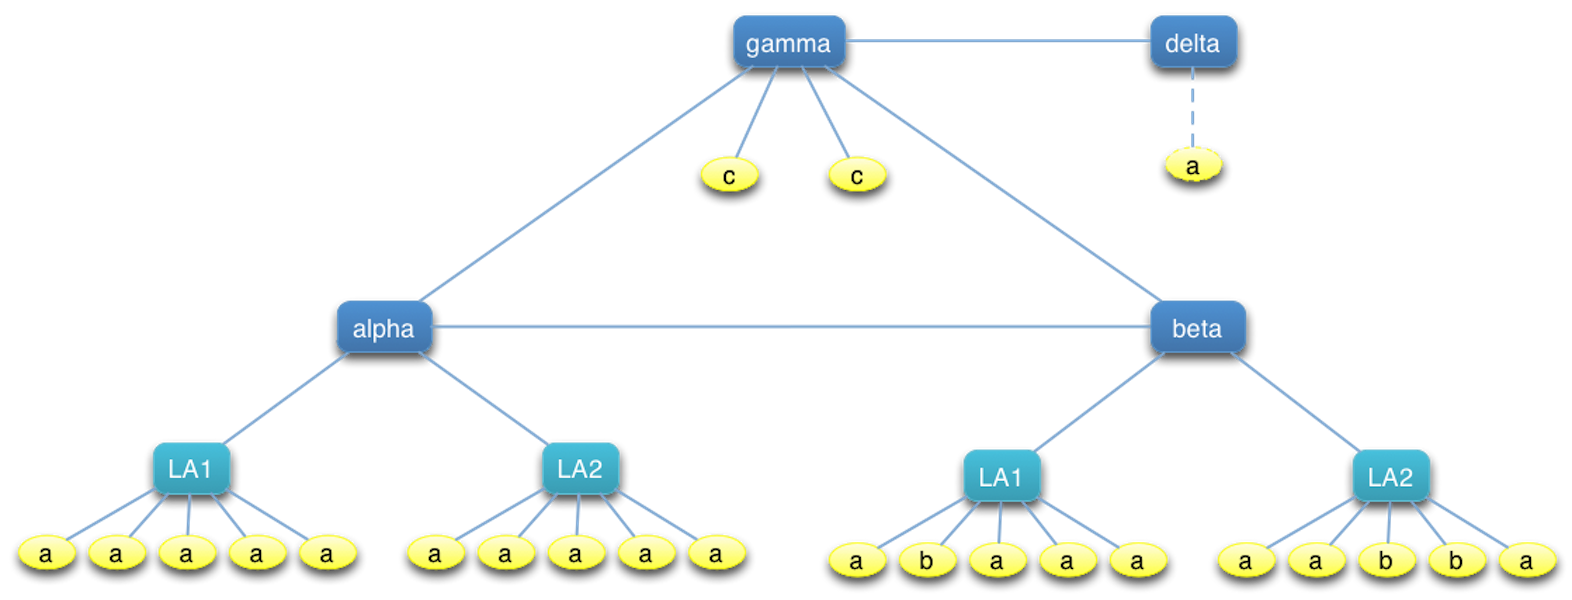
\includegraphics{fig/multima.eps}}
   \resizebox{.7\linewidth}{!}{
\includegraphics{fig/logo_DIET.ps}}
   \label{fig:multima}
  \caption{Example of a multi-MA deployment}
 \end{center}
\end{figure}

The following lines appear in the MA configuration file of alpha. They tell
that the multi-MA extension should listen for incoming connection at port
2001. They also tell that the MA should create a link toward the MA of the
organization gamma and toward the MA of the organization beta. (The description
of each configuration parameter are available in
section~\ref{sec:multimaconfig}).

\begin{verbatim}
agentType = DIET_MASTER_AGENT
dietHostname = diet.alpha.com
bindServicePort = 2001
neighbours = diet.beta.com:2001,ma.gamma.com:6000
\end{verbatim}

The following lines appear in the MA configuration file of beta:

\begin{verbatim}
agentType = DIET_MASTER_AGENT
dietHostname = diet.beta.com
bindServicePort = 2001
neighbours = diet.alpha.com:2001,ma.gamma.com:6000
\end{verbatim}

The following lines appear in the MA configuration file of gamma. The
\texttt{neighbours} value is empty. This means that the gamma's MA will not try
to connect itself to other MA. However, the three others are configured to be
connected to gamma. So, after all, the gamma MA is connected to the other
three.

\begin{verbatim}
agentType = DIET_MASTER_AGENT
dietHostname = ma.gamma.com
bindServicePort = 6000
neighbours = 
\end{verbatim}

Finally the following lines appear in the MA configuration file of delta:

\begin{verbatim}
agentType = DIET_MASTER_AGENT
dietHostname = ma.delta.com
bindServicePort = 2001
neighbours = ma.gamma.com:6000
\end{verbatim}

\section{Search examples}

The following section explained how a \texttt{diet\_call} is managed when used
on the previous architecture.

If a client sends a \texttt{diet\_call} for the problem \textbf{a} to the
alpha's MA, the alpha's MA will return a reference of one of it's SeD. However,
if its scheduler (see section~\ref{ch:plugin}) says that no SeD is available,
it will forward the request to beta and gamma. If beta has an available SeD, it
will be used to resolve the problem. If not, the request is forwarded to delta.

Now, if a client sends a \texttt{diet\_call} for the problem \textbf{c} to the
delta's MA. The delta MA does not have a SeD that can resolve this problem. So,
it forwards the request to gamma. If gamma has not available SeD, the request
is forwarded to alpha and beta.
